\subsubsection{Fundamental features}
\label{sec:methods_features_fundamental}

The dataset of bitcoin prices and volume comes with open, close, highest and
lowest daily prices, and volume expressed in transacted coins and their market
value in USD. Figures \ref{fig:btc_prices_all} and \ref{fig:btc_prices_split}
show the bitcoin daily prices. Figure \ref{fig:btc_volume} shows the volume
series.

\begin{figure}[H]
    \centering
    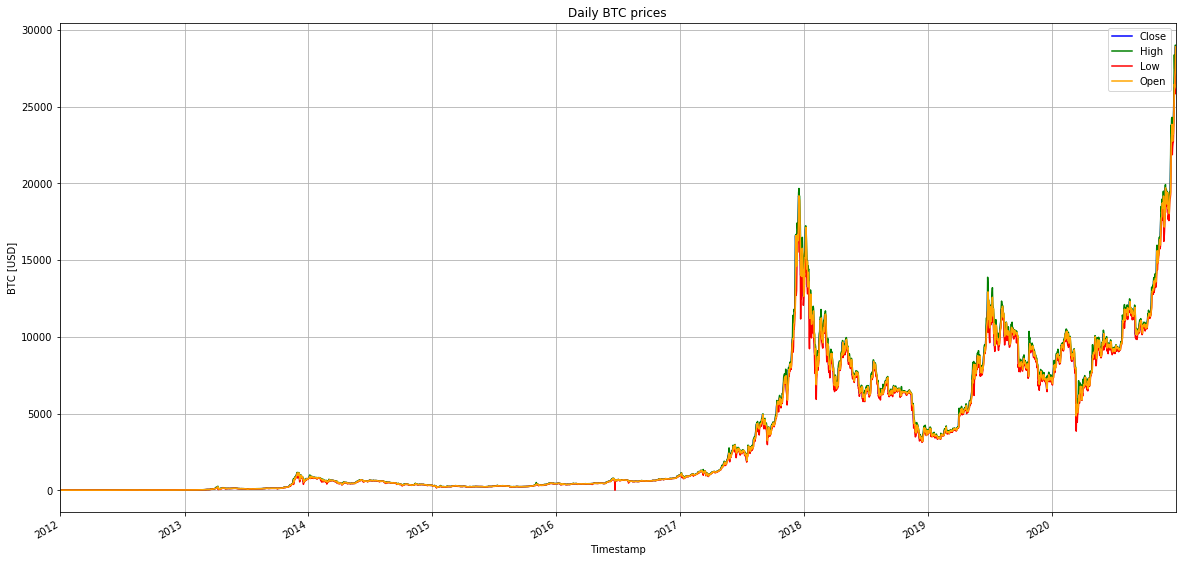
\includegraphics[width=\textwidth]{methods/images/btc_prices_all.png}
    \caption{Overlapped open, close, high and low bitcoin daily prices in USD.}
    \label{fig:btc_prices_all}
\end{figure}

\begin{figure}[H]
    \centering
    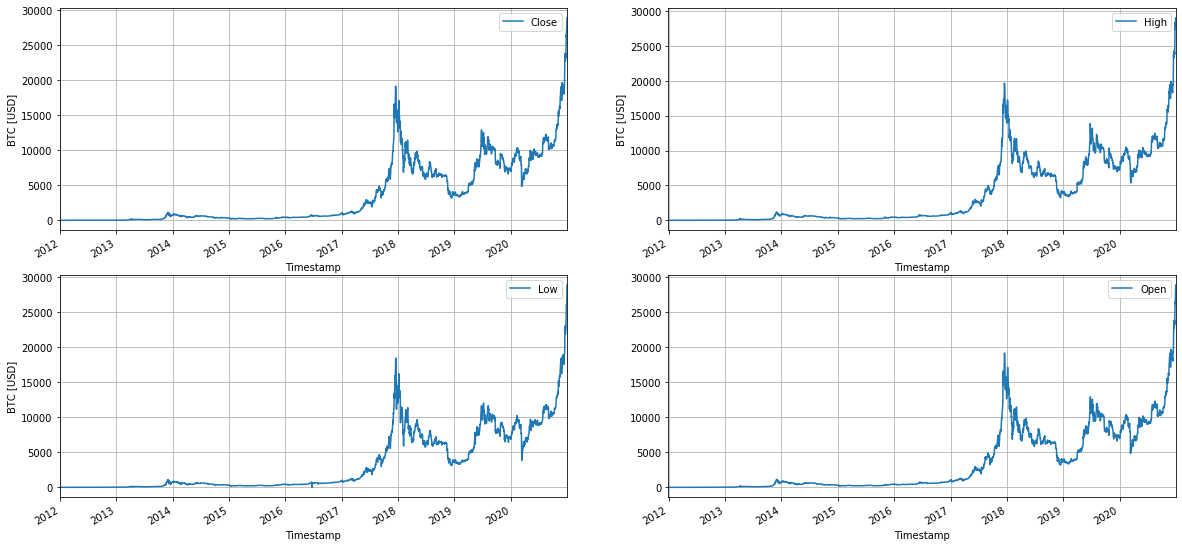
\includegraphics[width=\textwidth]{methods/images/btc_prices_split.png}
    \caption{Split of open, close, high and low bitcoin daily prices in USD.}
    \label{fig:btc_prices_split}
\end{figure}

\begin{figure}[H]
    \centering
    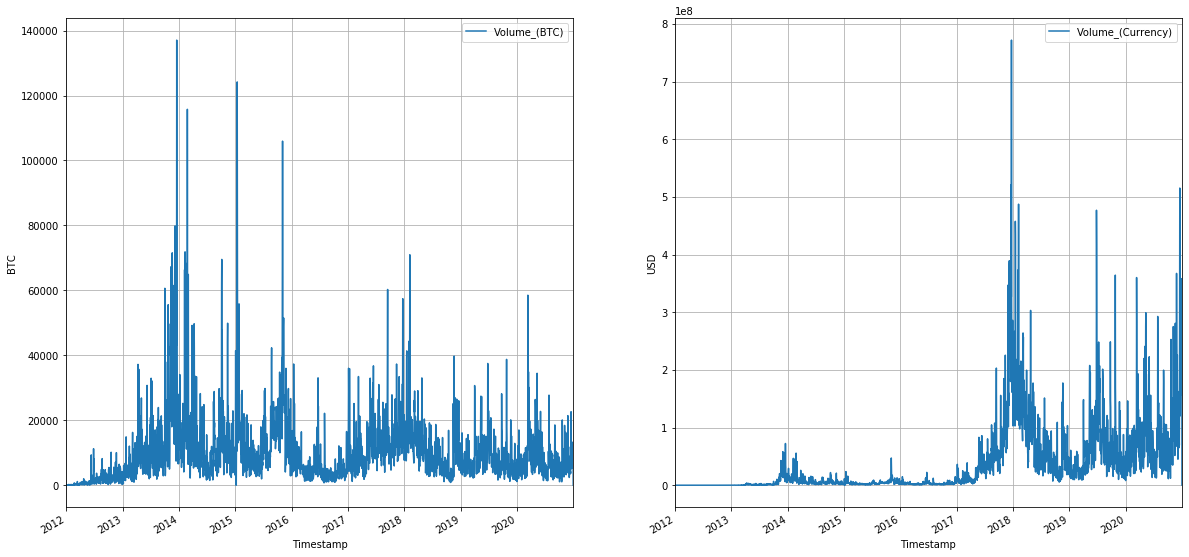
\includegraphics[width=\textwidth]{methods/images/btc_volume.png}
    \caption{The graph on the left shows the bitcoin daily volume. The graph on the right shows the market volume valuation in USD.}
    \label{fig:btc_volume}
\end{figure}

For volume series, the fractional differentiation was not enough so a log transformation
was added to stabilize the mean. Results can be seen in figure \ref{fig:btc_volume_log}.

\begin{figure}[!htb]
    \centering
    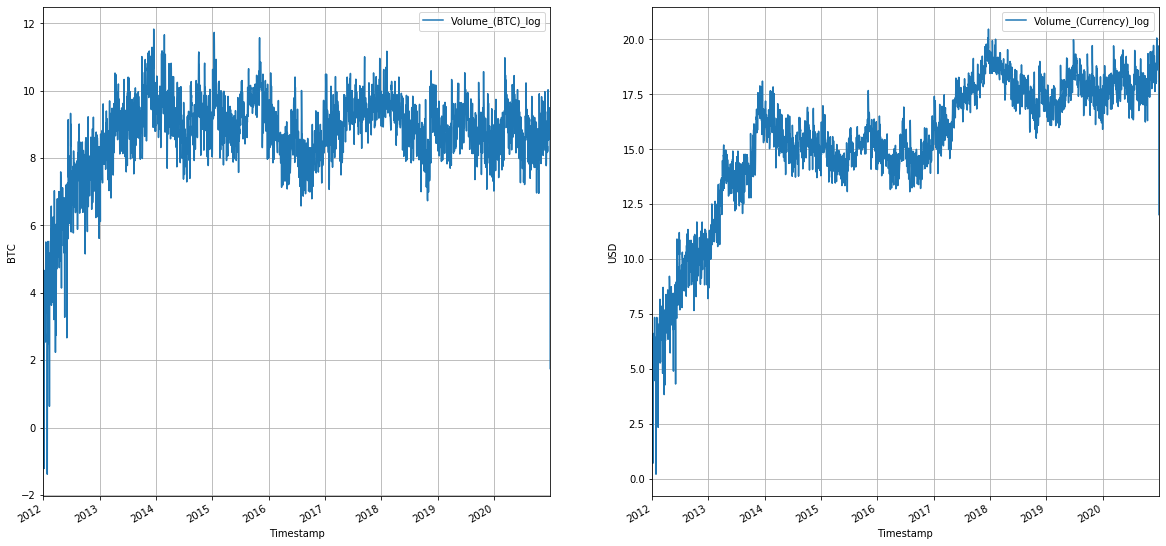
\includegraphics[width=\textwidth]{methods/images/btc_volume_log.png}
    \caption{Same features as in \ref{fig:btc_volume} but taking the logarithm.}
    \label{fig:btc_volume_log}
\end{figure}

Price series require fractional differentiation as explained in
\ref{sec:methods_features}. We could obtain the best $d^*$ for each price time
series applying the method previously described. Ten samples in the range
$[0, 1]$ are taken to look for the best $d^*$ which shields the results in table
\ref{table:frac_diff_prices}.

\begin{table}[!htb]
  \begin{center}
    \begin{tabular}{ | c | c | }
      \hline
      Feature & $d^*$ \\
      \hline
      Close   & 0.4   \\  
      \hline
      Open    & 0.4   \\
      \hline
      High    & 0.4   \\
      \hline
      Low     & 0.2   \\    
      \hline
    \end{tabular}
    \caption{Fractional differentiation order for price series.}
    \label{table:frac_diff_prices}
  \end{center}
\end{table}

Just for illustration purposes, see figure \ref{fig:close_ffd} that shows the
Close price series and the same series with an overlap of the fractionally
differentiated counterpart. Note the $y$ axis on the right which tracks the
scale of the fractionally differentiated Close price series. It can be seen
perfectly the effect of differentiating the series.

\begin{figure}[!htb]
    \centering
    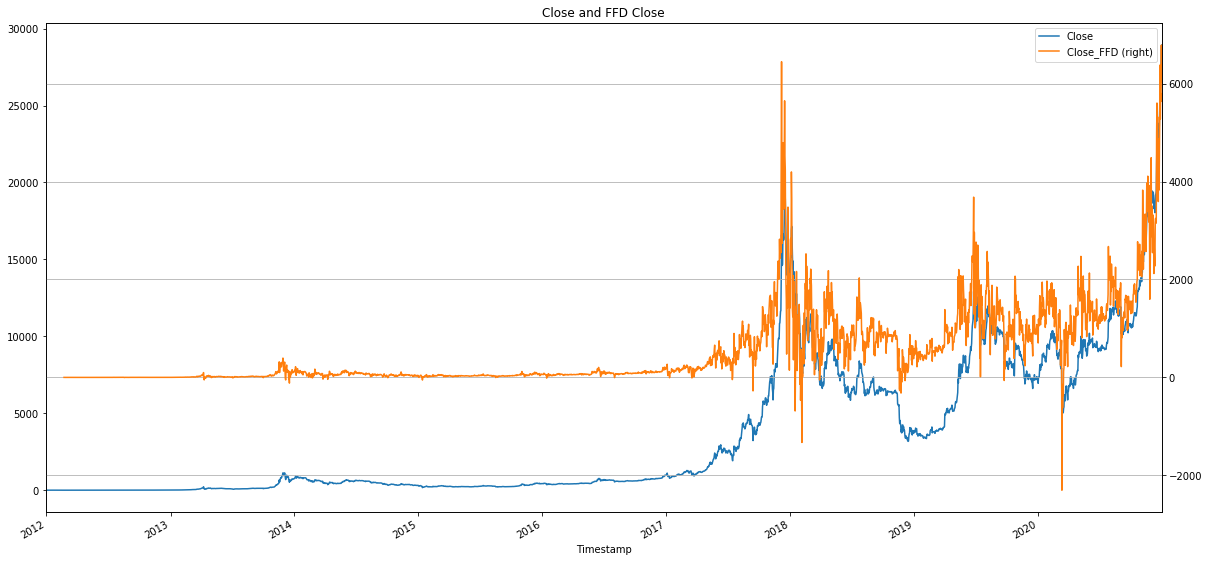
\includegraphics[width=\textwidth]{methods/images/btc_close_ffd.png}
    \caption{Close price and fractionally differentiated Close price with $d^* = 0.4$ (see table \ref{table:frac_diff_prices}).}
    \label{fig:close_ffd}
\end{figure}

On the other hand, other features were created out of the Close price series.
Those features features are:

\begin{itemize}
  \item RSI: Relative Strength Indicator. It is a momentum index that measures
        the strength or weakness of a stock price. Some time windows are used in
        favor of capturing high speed and low speed trends. See figure
        \ref{fig:rsi}.
  \item Autocorrelation: with different lags and time window lengths, the price
        series autocorrelation looks for repetitive patterns in the signal.
        Peaks in the autocorrelation signal indicate an occurrence of
        repetition. See figure \ref{fig:autocorrelation}
  \item Logarithm of the returns: just what the index expresses. It uses a
        logarithm transform to control the variance of the series. See figure
        \ref{fig:log_returns} and the histogram of values.
  \item Volatility: computed as the standard deviation of the moving average of
        the log returns. That yields the trend in return variation. Multiple
        time windows are used to capture different speeds. See figure
        \ref{fig:volatility}.
\end{itemize}

\begin{figure}[H]
    \centering
    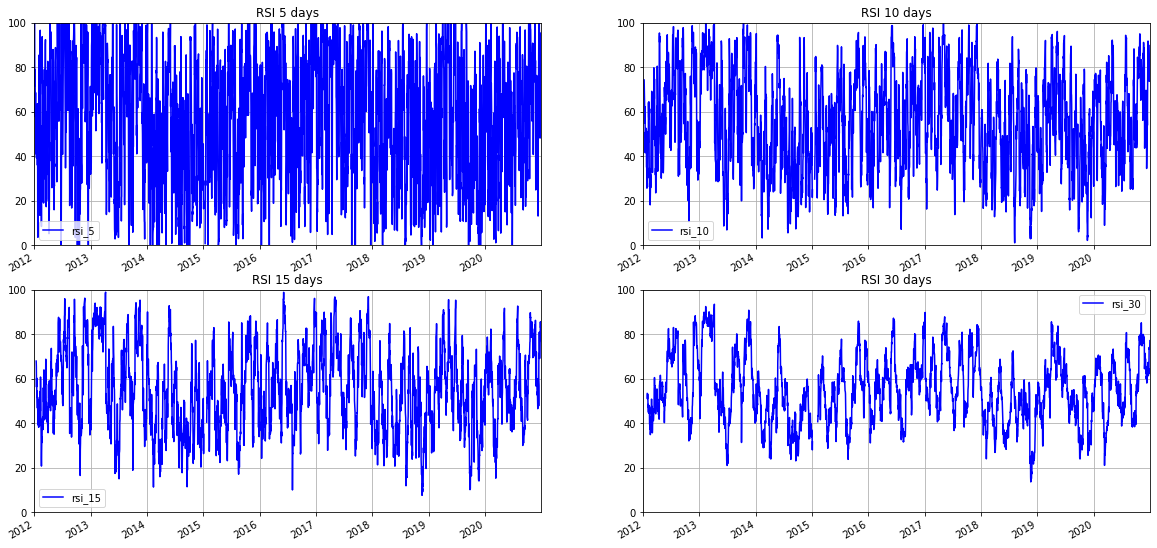
\includegraphics[width=\textwidth]{methods/images/rsi.png}
    \caption{RSI indexes for Close prices.}
    \label{fig:rsi}
\end{figure}

\begin{figure}[H]
    \centering
    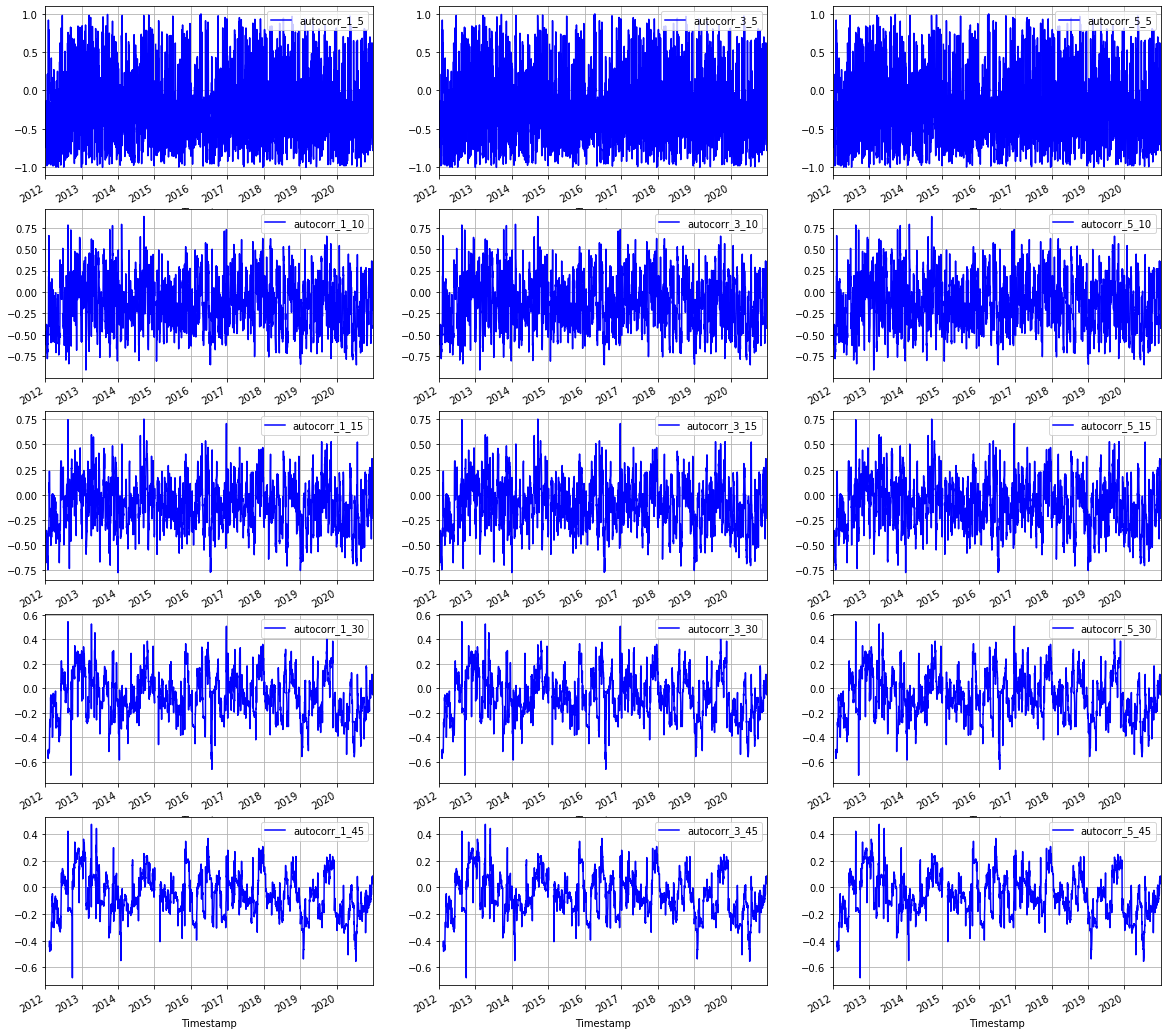
\includegraphics[width=\textwidth]{methods/images/autocorrelation.png}
    \caption{Different autocorrelation signals with different lags and time
    windows.}
    \label{fig:autocorrelation}
\end{figure}

\begin{figure}[H]
    \centering
    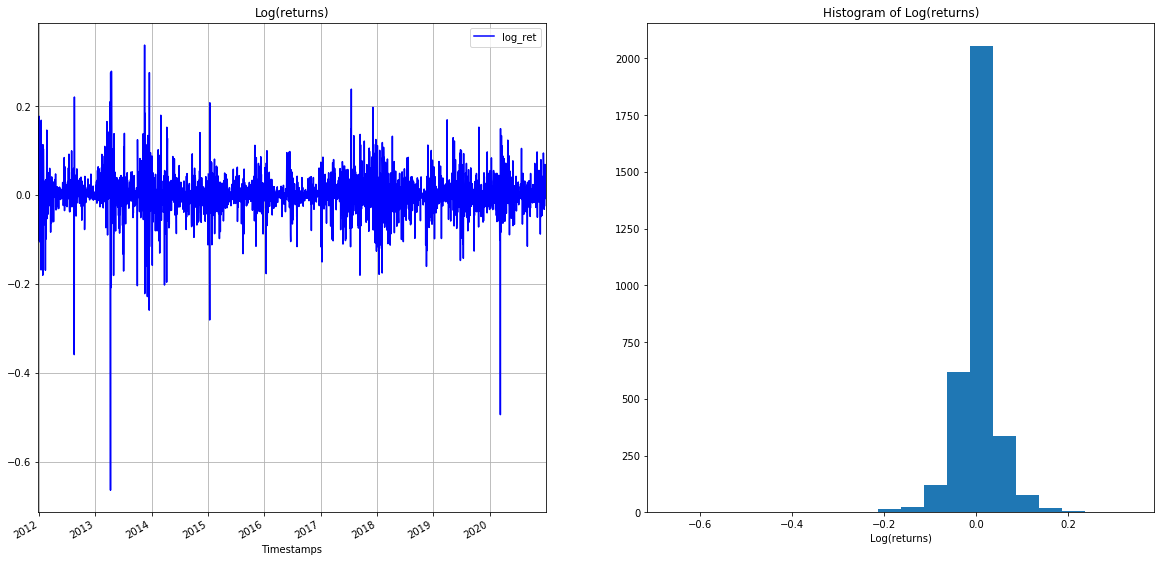
\includegraphics[width=\textwidth]{methods/images/log_returns.png}
    \caption{Logarithm of returns on the left, the histogram of the logarithm of returns on the right.}
    \label{fig:log_returns}
\end{figure}

\begin{figure}[H]
    \centering
    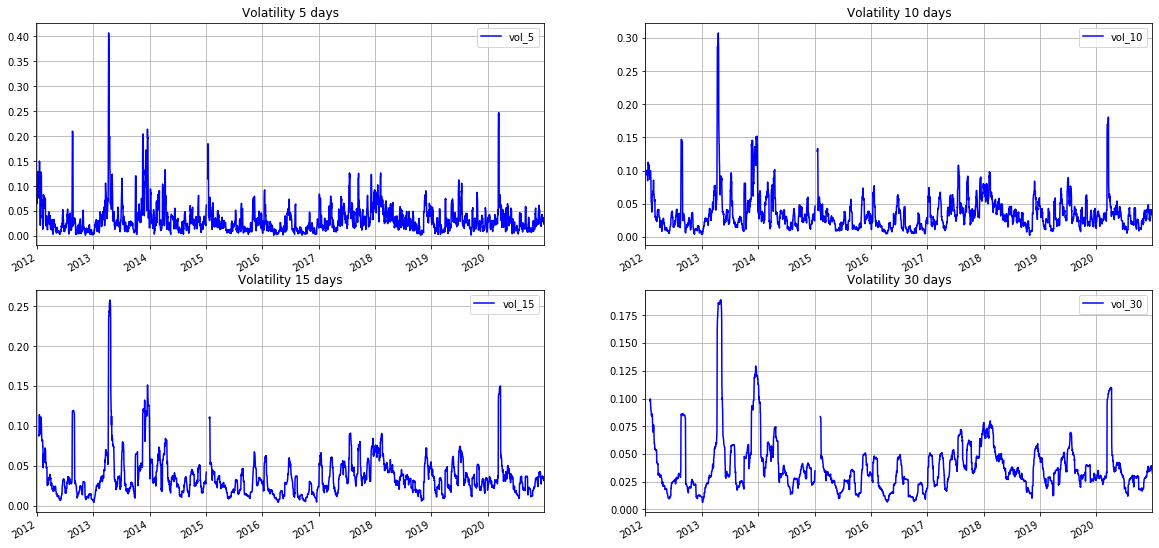
\includegraphics[width=\textwidth]{methods/images/volatility.png}
    \caption{Volatility index.}
    \label{fig:volatility}
\end{figure}